\documentclass[UTF8]{ctexart}
\usepackage{amsmath}
\usepackage{diagbox}
\usepackage{textcomp}
\usepackage{graphicx}
\usepackage{float}
\usepackage{caption}
\usepackage{adjustbox}
\usepackage{subfigure}
\usepackage{geometry}
\usepackage{pifont}
\usepackage{gensymb}
\usepackage{bm}
\begin{document}
\renewcommand{\thefootnote}{\fnsymbol{footnote}}
\newgeometry{left=2cm,bottom=4cm,right=2cm}
\linespread{1.4}
\title{\vspace{-5em}\heiti光栅衍射实验报告\vspace{-2.5em}}
\date{}
\maketitle
\begin{center}
{\fangsong 徐浩博\quad 基科01\quad2020010108}
\end{center}

\subsubsection*{摘要}
{\kaishu\normalsize  本实验旨在通过分光计的调节和对光栅衍射等实验现象的观察,测量出光栅常数和光波波长,使我掌握了分光计的基本使用方法,学会了利用自准直法调节实验条件,并对用正入射、斜入射、最小偏向角等相关知识测量光波波长的三种方法有了更深的理解. 同时,我还通过相关计算进一步巩固了实验误差的分析、不确定度等相关知识.}
\subsubsection*{关键词:分光计\quad光栅\quad衍射\quad双面反射镜\quad光栅常数\quad正入射\quad斜入射\quad最小偏向角\quad \vspace{1.5em}}

\section{实验仪器}
本实验用到的主要仪器有:\par
1) 分光计\par
2) 汞灯\par
3) 双面反射镜、光栅

\section{实验原理及实验数据}

\subsection*{ 1. 分光计的调节}
\subsubsection*{1.1 粗调}
粗调分光仪,应旋转平行光管和望远镜的抚养角调节螺钉,使平行光管和望远镜平行于刻度盘;同时目测并旋转载物台下的三个水平螺钉,使载物台上下两层近似平行,缝宽不过大也不过小. 缝过宽或过窄都会导致螺钉调节的余地过小. 如此便完成了粗调.

\subsubsection*{1.2 调节望远镜至适合观察平行光}
1)旋转望远镜目镜套筒,调节目镜与叉丝的距离直至可以看清分划板上的十字叉丝像. 此时分划板位于目镜的一倍焦距处.\par
2)将双面反射镜放置于载物台上,如下图所示:

\begin{figure}[H]\begin{center}
    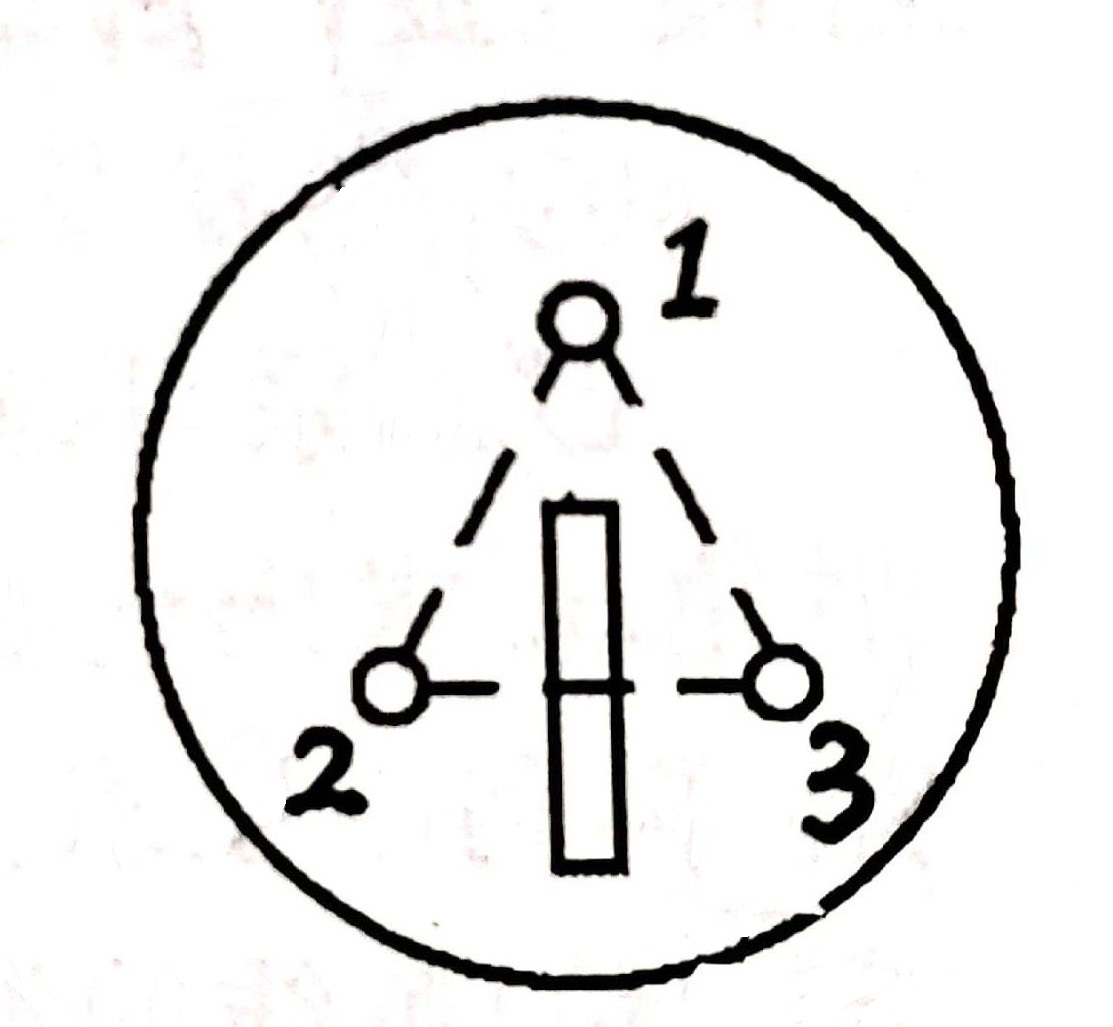
\includegraphics[scale=0.2]{1.jpg}
    \caption{反射镜摆放示意图}
\end{center}\end{figure}

旋转载物台直至平面镜与望远镜光轴垂直,若粗调适当,则此时可以在望远镜中看到明亮的绿色十字光斑;若无法找到则需进一步粗调.\par
3)旋转望远镜调焦旋钮,改变物镜到分划板间的距离,调节到绿色十字像最清晰为止,此时分划板大约位于物镜的一倍焦距处.\par
4)待以上工作进行完成后,我们上下左右移动视线,观察绿色十字像是否移动. 若移动则再进行分划板与目镜、物镜间的距离调节;若十字像不再移动,则说明实验已经基本消除了视差. 消除视差对此实验十分重要,因为通过望远镜观察各种像时,眼睛与目镜的相对位置可能会发生一定改变,而如果存在视差,则该改变会导致人们无法准确找到像的位置;而分光计是较为灵敏的仪器,像的位置发生微小的改变,会导致测量结果也产生较大偏差. 综上,消除视差对于实验来讲是十分重要的.

\subsubsection*{1.3 调节望远镜光轴垂直于分光计主轴}

旋转载物台180度后,在望远镜中观察是否还能看到双面反射镜反射回的绿色叉丝像,若无法观察,则重新进行粗调并保证可以在望远镜中观察到双面反射镜两个面反射回的绿色叉丝像. 此后,应当采用渐进法进行进一步调节.\par
具体来说,在双面反射镜某一面反射时,旋转载物台使绿色叉丝像在竖直方向对准分划板叉丝. 若绿色十字像与分划板╪ 形叉丝上十字不重合,则先调节载物台下的水平螺钉2或3,使得绿色十字像与分划板╪ 形叉丝上十字间的距离减小一半,再调节望远镜俯仰角调节螺钉,使得绿色十字像与分划板╪ 形叉丝上十字重合. 然后,再将双面反射镜旋转180度,用渐进法进行同样调节. 如此反复几次,可以做到双面反射镜的两个面反射时,绿色十字像都与╪ 形叉丝上十字重合,则望远镜光轴已垂直于分光计主轴.\par
我们首先回答一个问题:为何需要绿色十字像与╪ 形叉丝上十字重合. 如下图,
\begin{figure}[H]\centering
    {
    \subfigure[十字叉丝成像光路图]{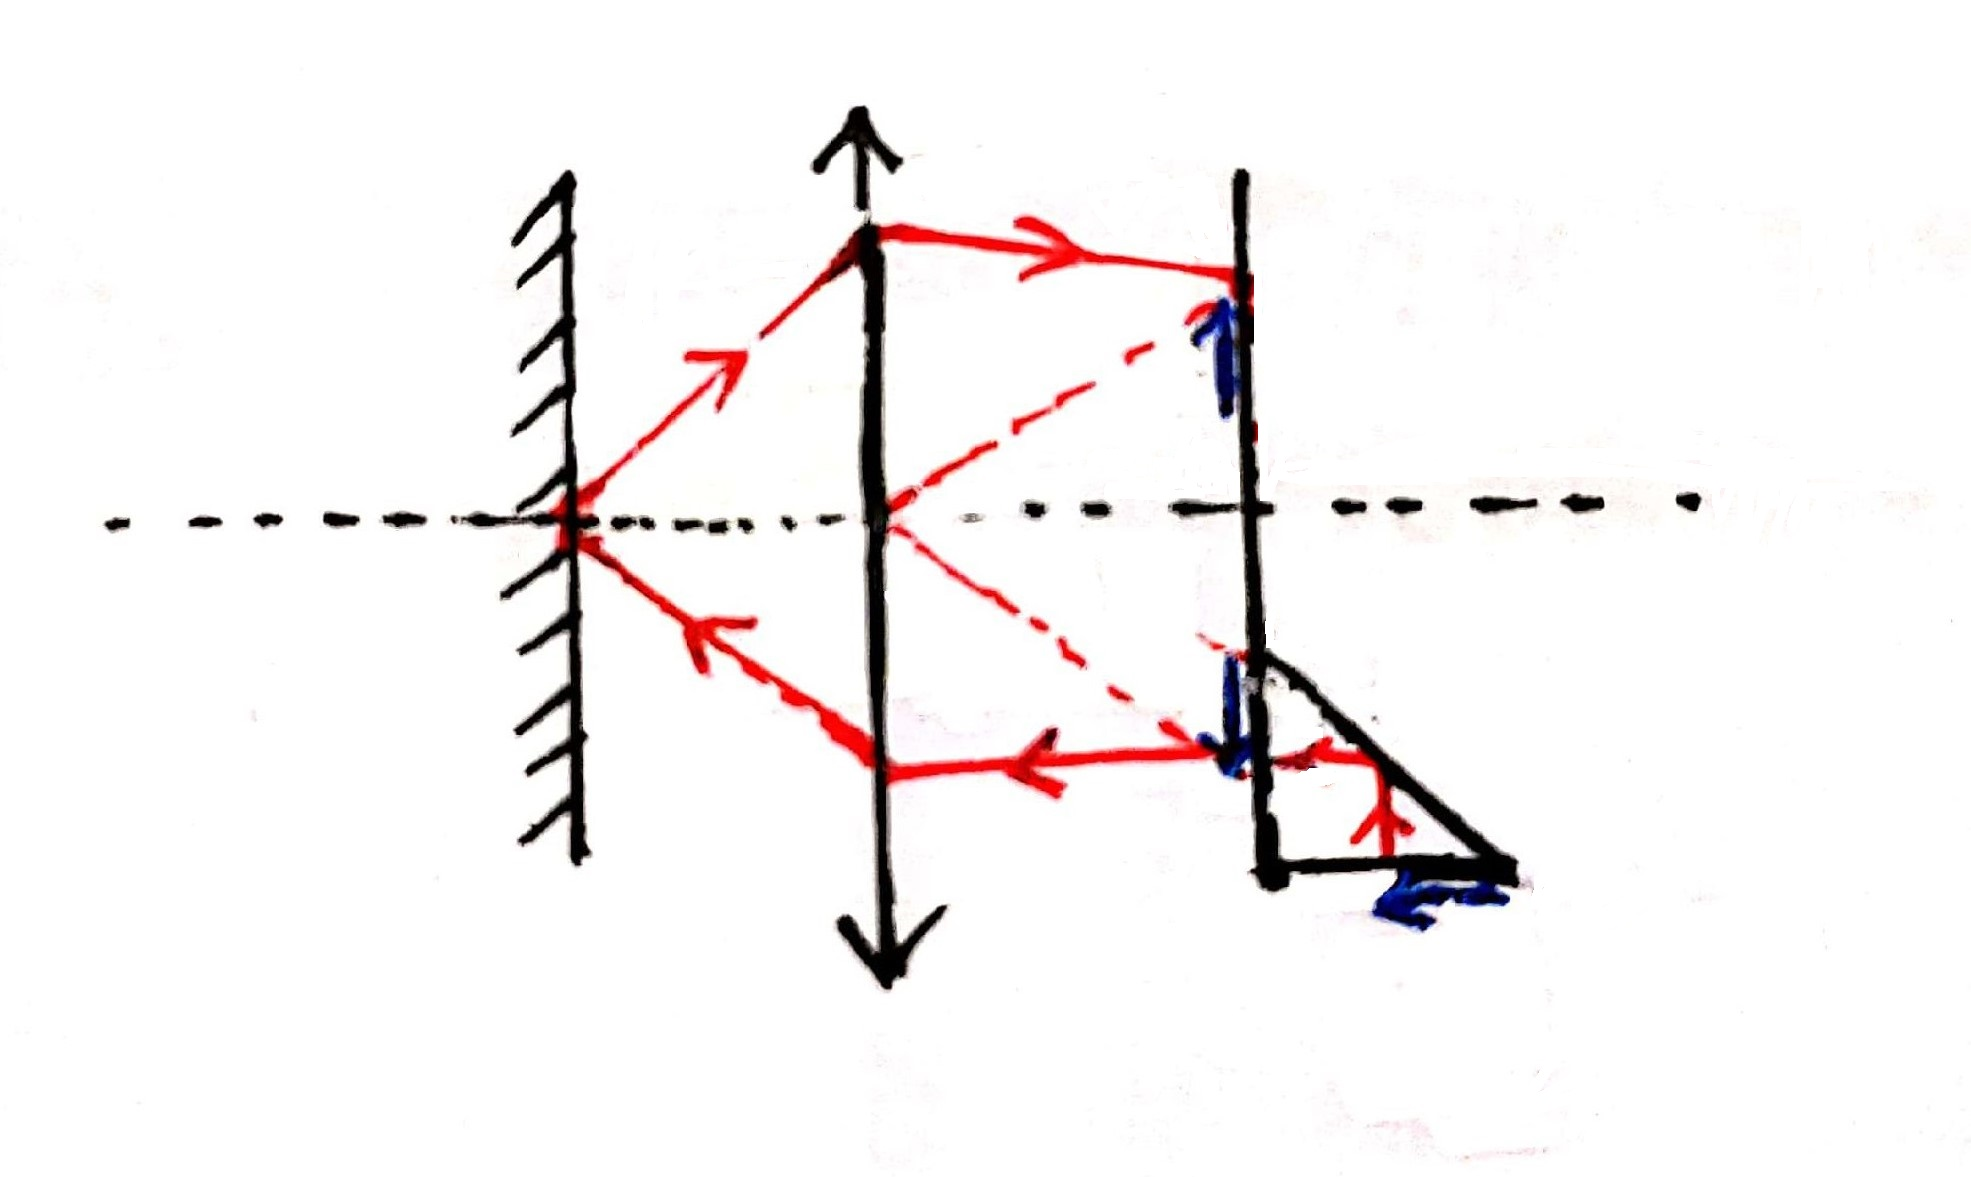
\includegraphics[scale=0.15]{2.jpg}}\hspace{20mm}
    \subfigure[分划板上叉丝反射像示意图]{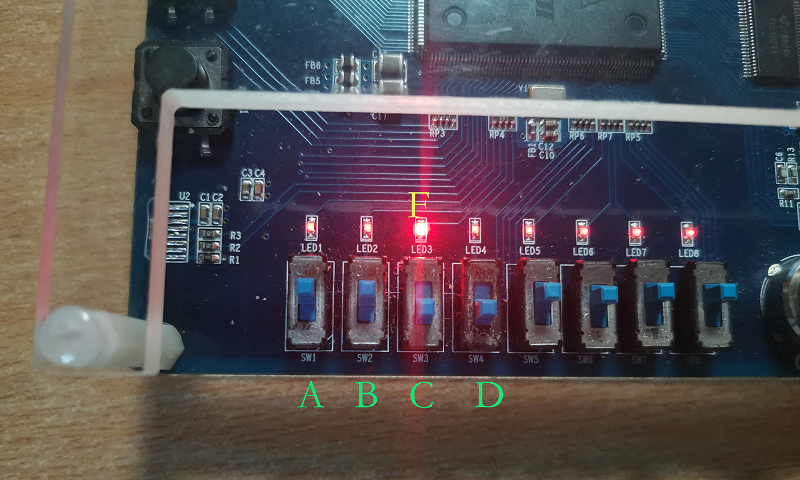
\includegraphics[scale=0.96]{3.png}}
    \caption{自准直法原理图}
    }
    \end{figure}
我们发现棱镜反射的十字形透光叉丝的像与双面反射镜反射回的绿色十字像分距分划板中心的两侧. 十字形透光叉丝要经过棱镜、反射镜、物镜三次成像. 考虑到在分光计的构造中,小棱镜面紧贴分划板,且棱镜对称,则十字透光叉丝经过棱镜恰好成像在分划板上;设分划板到反射镜距离为d,若反射镜与分划板平行,则可认为反射镜将棱镜成的像投射至距离反射镜d的后方. 对于物镜来说,物是反射镜中的像,设其中心点距离光轴中心距离为y;由于物距与像距均为d,则根据对称性,像的中心点距离光轴中心距离也为y. 这说明,在理想情况下,棱镜反射的十字形透光叉丝的像与双面反射镜反射回的绿色十字像分距分划板中心的两侧,即绿色十字像与╪ 形叉丝上十字重合,而这一点实际上需要满足反射镜与分划板平行(即反射镜与望远镜主轴垂直)这一条件;因此,调节绿色十字像都与╪ 形叉丝上十字重合,实际上就是在调节反射镜与望远镜主轴垂直.\par
如下图,若反射镜正反两面都与望远镜主轴垂直,则有∠1=90°,∠2=90°,因此∠1=∠2=90°,则望远镜光轴已已垂直于分光计主轴. 这也就是为什么我们要保证旋转180°后,绿色叉丝像仍要与╪ 形叉丝上十字重合的缘故.
\subsubsection*{1.4 调节平行光管}
取下反射镜. 首先旋转平行光管调焦旋钮,调整狭缝与望远镜间距离,使得透过平行光管的光线能够汇聚到望远镜分划板上.\par
其次调整平行光管后方狭缝宽度,使得狭缝宽度适宜.\par
最后调节平行光管俯仰角螺钉,使得在望远镜中平行光管的像被分划板中心叉丝横线平分为两半,此时平行光管已垂直于主轴.

\subsection*{ 2. 光线垂直入射时,测定光栅常数和光波波长}
\subsubsection*{2.1 调节光栅平面与平行光管光轴垂直}
将光栅如图1一样摆放. 由于光栅炮制工艺问题,光栅两面平面与细缝未必完全平行,因此可以选择反射绿色十字像较亮的一面朝向望远镜,另一面接受入射光.\par
调节光栅平面与平行光管光轴垂直时,只需采用自准直法,在平行光管狭缝像位于望远镜分划板中央竖直线上时,旋转载物台,使得绿十字像中心也位于分划板竖直线上,此时观察绿十字像中心是否位于分划板╪ 形叉丝上十字,如果存在偏差,则调节载物台水平螺丝2或3. 调节完成后,若绿十字像歪斜,则调节水平螺丝1,直至绿十字像与分划板╪ 形叉丝上十字完全重合. 若平行光管、分划板上叉丝和平行光管三像合一,则此时光栅平面与平行光管光轴垂直.

\subsubsection*{2.2 调节光栅刻线与分光计主轴平行}
考虑到光栅有两个自由度,即俯仰、左右,2.1已调整好俯仰,则左右角度调整时,旋转载物台水平螺丝1,保证各级衍射谱线等高即可. 注意,旋转水平螺丝1时可能会导致俯仰也出现微小的改变,此时需要返回2.1再次调整俯仰角度. 待调整所有衍射谱线等高后,光栅刻线与分光计主轴平行.\par
下面在正式实验前,我们再进行一步验证,即验证此时平行光管光线的确为垂直入射. 具体来说,我们测量中心主极大的方位$\phi_0$,再分别测量-2级外侧黄光(左)的方位$\phi_-$与+2级外侧黄光(右)的方位$\phi_+$,并计算夹角分别为$\Delta\phi_-=\Big{|}\phi_--\phi_0\Big{|}$、$\Delta\phi_+=\Big{|}\phi_+-\phi_0\Big{|}$,若夹角之差在2'之内,则认为入射光垂直于光栅平面.\par
考虑到刻度盘具有偏心差,因此我们采用左右游标分别读数再取平均值的方法获得方位. 设左右游标读数分别为$\phi_1$、$\phi_2$,则方位可以认为是$\displaystyle{\phi=\frac{\phi_1+\phi_2}{2}}$.\\ \par
实验数据如下:
\begin{table}[H]\begin{center}
    \caption{光线垂直入射预实验数据记录表}
    \begin{tabular}{|c|c|c|c|}
        \hline
        衍射线级数&左游标读数$\phi_1$&右游标读数$\phi_2$&平均读数$\phi=(\phi_1+\phi_2)/2$\\
        \hline
        $m=-2$&	145°25′ &325°26′&	235°25′\\
        \hline
        $m=0$	&	125°06′ &305°04′	&215°05′\\
        \hline
        $m=2$	&	104°45′& 284°46′&	194°45′\\
        \hline        
    \end{tabular}
\end{center}\end{table}
则外侧黄光-2级与0级夹角为$\Delta\phi_-=\Big{|}\phi_--\phi_0\Big{|}=\Big{|}235\degree25'-215\degree05'\Big{|}=20\degree20'$,+2级与0级夹角为$\Delta\phi_+=\Big{|}\phi_+-\phi_0\Big{|}=\Big{|}194\degree45'-215\degree05'\Big{|}=20\degree20'$,两者差为0',可以看出,此时平行光管光线的确为垂直入射.

\subsubsection*{2.3 测量光栅常数和光波波长的理论推导}

\begin{figure}[H]\begin{center}
    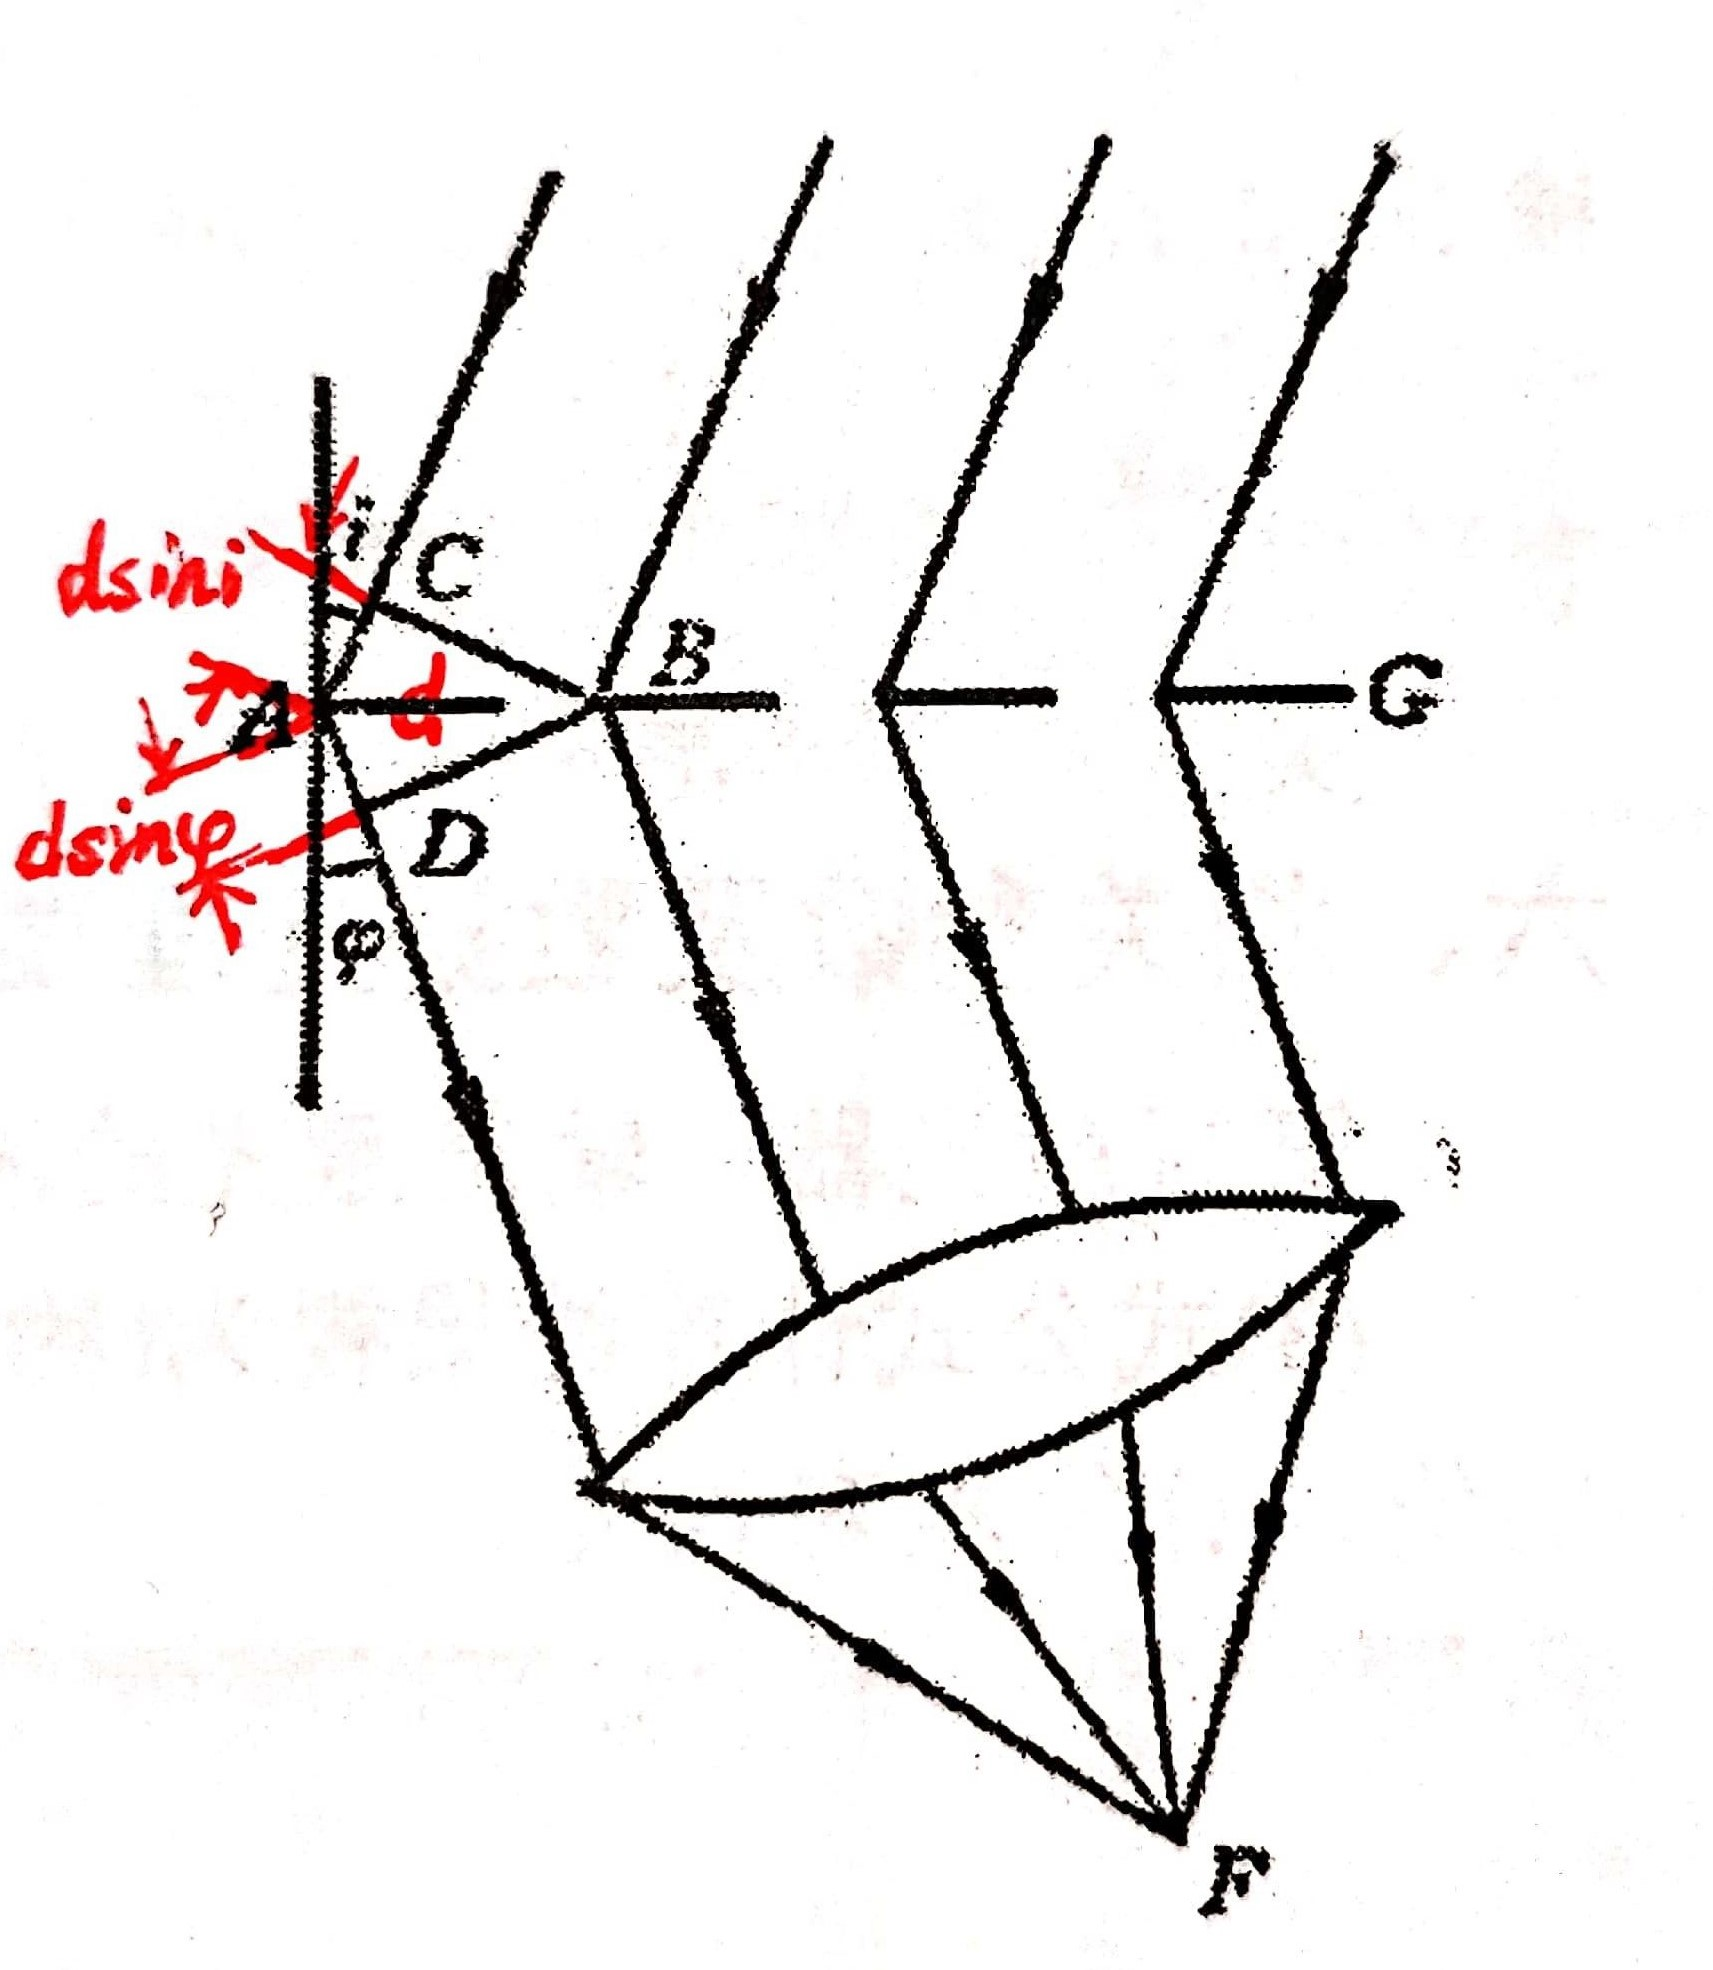
\includegraphics[scale=0.16]{4.jpg}
    \caption{光栅衍射原理图}
\end{center}\end{figure}

如图,通过光栅相邻两个刻缝的光线光程差为
\begin{equation}
    \label{yanshe}
    d(\sin i\pm\sin \phi)=m\lambda
\end{equation}
其中$d$为光栅常数(刻缝间距),$i$为入射角,$\phi$为衍射角,$m$为衍射级数,$\lambda$为光波波长. 当衍射角与入射角位于法线同侧时,等式取正号;异侧则取负号.\par
在正入射条件下,$i=0$,则有
\begin{equation}
    \label{zhengrushe1}
    d\sin\phi_m=m\lambda
\end{equation}\par
为了提高精度,可以测量零级左右两侧对应级次的衍射线夹角$2\phi_m$. 具体测量时,设左右两个衍射线方位分别为$\phi_2$,$\phi_1$,不妨设$\phi_2>\phi_1$,则有$2\phi_m=\phi_2-\phi_1$,如此,则(\ref{zhengrushe1})式可改写为
\begin{equation}
    \label{zhengrushe2}
    d\sin\frac{\phi_2-\phi_1}{2}=m\lambda
\end{equation}\\
测量光栅常数时,我们采用绿光的约定真值$\lambda_{GN}=546.1nm$,并测量绿光的左右$m$级衍射线对应方位$\phi_{20}$,$\phi_{10}$,则有
\begin{equation}
    \label{d}
    d=\frac{m\lambda_{GN}}{\sin\phi_0}=\frac{m\lambda_{GN}}{\sin\frac{\phi_{20}-\phi_{10}}{2}}
\end{equation}
得到光栅常数$d$,我们再测量波长较小的黄光的左右$m$级衍射线对应方位$\phi_2$,$\phi_1$,则有
\begin{equation}
    \label{lambda}
    \lambda=\frac{d\sin\phi_m}{m}=\frac{d\sin\frac{\phi_{2}-\phi_{1}}{2}}{m}
\end{equation}\\

\hspace{-2em}下面进行不确定度计算:\par
约定一次测量时,忽略$\phi_1$、$\phi_2$的A类不确定度,而二者通过$\phi_{10}=(\phi_{11}+\phi_{12})/2$、$\phi_{20}=(\phi_{21}+\phi_{22})/2$计算而得. $U_{ij}=U_B\approx\Delta_{INS}$,则二者不确定度约为$\displaystyle{U_{\phi_{10}}=U_{\phi_{20}}=\frac{\sqrt2}{2}U_{ij}=\frac{\sqrt2}{2}\Delta_{INS}}$. 然而我们有\\$\phi_m=(\phi_{20}-\phi_{10})/2$,因此$\displaystyle{U_{\phi_m}=\frac{\sqrt2}{2}U_{10}=\frac{\Delta_{INS}}{2}}$. 不确定度计算公式为
\begin{equation}
    \label{buquedingdu}
    U=\sqrt{(\frac{\partial y}{\partial x_1}U_{x_1})^2+(\frac{\partial y}{\partial x_2}U_{x_2})^2+\cdots}
\end{equation}
因此计算光栅常数时,结合(\ref{d})式,有
\begin{equation}\begin{split}
    U_d&=
    \sqrt{(\frac{\partial d}{\partial \phi_{m}}U_{\phi_{m}})^2}\\
    &=\sqrt{
        (\frac{m\lambda_{GN}\cos\phi_m}
        {\sin^2\phi_m}\frac{\Delta_{INS}}{2})^2}\\
    &=\frac{\Delta_{INS}}{2}d \cot\phi_m
\end{split}\end{equation}
由上式可知,$\displaystyle{\cot\phi_m}$越小,即$\phi_m$越大,也即$m$越大时,$d$的不确定度越小. 但$m$越大,衍射条纹也就越暗,同时,还有可能与更高级次的衍射线交叉、重合. 综合以上,我们选取$m=\pm3$的绿色衍射线来进行测量.\par
再由(\ref{buquedingdu})式和(\ref{lambda})式,我们可以推导$\lambda$的不确定度
\begin{equation}\begin{split}
    U_{\lambda}&=
    \sqrt{(\frac{\partial \lambda}{\partial \phi_{m}}U_{\phi_{m}})^2+(\frac{\partial \lambda}{\partial \phi_{2}}U_{\phi_{2}})^2+(\frac{\partial \lambda}{\partial d}U_d)^2}\\
    &=\sqrt{(\frac{d\cos\phi_m}{m}U_{\phi_{m}})^2+(\frac{\sin\phi_m}{m}U_d)^2}\\
    &=\sqrt{(\frac{d\cos\phi_m}{m}\frac{\Delta_{INS}}{2})^2+(\frac{\sin\phi_m}{m}U_d)^2}\\
    &=\sqrt{(\frac{\Delta_{INS}\lambda \cot\phi_m}{2})^2+(\lambda\frac{U_d}{d})^2}
\end{split}\end{equation}
由上式可知,$\displaystyle{\cot\phi_m}$越小,即$\phi_m$越大,也即$m$越大时,$\lambda$的不确定度越小. 但$m$越大,衍射条纹也就越暗,同时,还有可能与更高级次的衍射线交叉、重合. 综合以上,我们选取$m=\pm3$的外侧黄光衍射线来进行测量.\par

\subsubsection*{2.4 测量光栅常数}
由(\ref{d})式,结合2.3知,在2.2确定的正入射的条件下,我们只需测量零级左右两侧第三级绿光衍射线位置,即可获知光栅常数.\par
测量数据如下:
\\\par
\begin{center}
保持测零级主极大位置时左游标读数125°06′,右游标读数305°04′,平均读数215°05′\vspace{-1em}
\end{center}
\begin{table}[H]\begin{center}
    \caption{光线垂直入射测量光栅常数数据记录表}
    \begin{tabular}{|c|c|c|c|}
        \hline
        衍射线级数&左游标读数$\phi_1$&右游标读数$\phi_2$&平均读数$\phi_m=(\phi_1+\phi_2)/2$\\
        \hline
        $m=-3$&	154°32′ &334°32′&	244°32′\\
        \hline
        $m=3$	&	95°36′& 275°35′&	185°35′\\
        \hline        
    \end{tabular}
\end{center}\end{table}
计算光栅常数为\\
\[d=\frac{m\lambda_{GN}}{\sin\phi_0}=\frac{m\lambda_{GN}}{\sin\frac{\phi_{20}-\phi_{10}}{2}}=\frac{3\times546.1nm}{\sin\frac{244\degree32'-185\degree35'}{2}}=3329.6nm\]
\[U_d=\frac{\Delta_{INS}}{2}d \cot\phi_m=\frac{2.9\times10^{-4}}{2}\times3329.6\times\cot{\frac{244\degree32'-185\degree35'}{2}}nm=0.85nm\]\\
因此,测得的光栅常数为$(3329.6\pm0.9)nm$.

\subsubsection*{2.5 测量黄光波长}
由(\ref{lambda})式,结合2.3知,在2.2确定的正入射的条件下,我们只需测量零级左右两侧第三级外侧黄光衍射线位置,即可获知该黄光的波长.\par
测量数据如下:
\\\par
\begin{center}
保持测零级主极大位置时左游标读数125°06′,右游标读数305°04′,平均读数215°05′\vspace{-1em}
\end{center}
\begin{table}[H]\begin{center}
    \caption{光线垂直入射测量黄光波长数据记录表}
    \begin{tabular}{|c|c|c|c|}
        \hline
        衍射线级数&左游标读数$\phi_1$&右游标读数$\phi_2$&平均读数$\phi_m=(\phi_1+\phi_2)/2$\\
        \hline
        $m=-3$&	156°33′&336°31′&246°32′\\
        \hline
        $m=3$&	93°37′&273°36′&183°36′\\
        \hline        
    \end{tabular}
\end{center}\end{table}
计算黄光波长为\\
\[\lambda=\frac{d\sin\phi_m}{m}=\frac{d\sin\frac{\phi_{2}-\phi_{1}}{2}}{m}=\frac{3329.6\times\sin\frac{246\degree32'-183\degree36'}{2}}{3}=579.4nm\]
\begin{equation}\nonumber\begin{split}
U_{\lambda}&=\sqrt{(\frac{\Delta_{INS}\lambda \cot\phi_m}{2})^2+(\lambda\frac{U_d}{d})^2}\\&=\sqrt{(\frac{2.9\times10^{-4}}{2}\times579.4\times\cot\frac{246\degree32'-183\degree36'}{2})^2+(579.4\times\frac{0.9}{3329.6})^2}nm=0.21nm
\end{split}\end{equation}
因此,测得的黄光波长为$(579.4\pm0.2)nm$. 这与黄光的约定真值$579.1nm$吻合得很好.

\subsection*{ 3. 光线15\degree角入射时,测定光波波长}

\subsubsection*{3.1 调整入射角}
保持平行光管的像位置为刻度盘左游标读数125°06′,右游标读数305°04′,平均读数215°05′,此时转动望远镜15\degree0',使得左右两个游标平均读数为230°05'或200°05'. 之后,转动载物台,用自准直法,使得光栅转动直至光栅平面反射回的绿色十字叉丝像与望远镜分划板╪ 形叉丝上十字重合,此时入射角为15°0'.\par
实际实验中,我调整望远镜,使得刻度盘左游标140°06′,右游标320°04′,平均读数$\phi_0=$230°05′.

\subsubsection*{3.2 理论推导}
根据(\ref{yanshe})式,有
\begin{equation}
    \lambda=\frac{d(\sin i\pm \sin \phi)}{m}=\frac{|d(\sin i\pm \sin \phi)|}{|m|}
\end{equation}
以入射光同侧为正,入射光异侧为负. 因此,已知法线的位置$\phi_0$,分别测量$\pm3$级黄光的位置$\phi_1$、$\phi_2$,即可知道左右3级衍射线与法线夹角$\Big{|}\phi_-\Big{|}=\Big{|}\phi_1-\phi_0\Big{|}$、$\Big{|}\phi_+\Big{|}=\Big{|}\phi_2-\phi_0\Big{|}$,以此再通过上式计算出黄光波长.

\subsubsection*{3.3 进行实验}
测量数据如下:\\
\begin{center}
    保持测量平行光管位置时左游标读数125°06′,右游标读数305°04′,平均读数215°05′\\
    保持自准直法测光栅法线位置时左游标140°06′,右游标320°04′,平均读数230°05′\vspace{-1em}
\end{center}
\begin{table}[H]\begin{center}
    \caption{光线垂直入射测量黄光波长数据记录表}
    \begin{tabular}{|c|c|c|c|}
        \hline
        衍射线级数&左游标读数$\theta_1$&右游标读数$\theta_2$&平均读数$\phi_i=(\theta_1+\theta_2)/2$\\
        \hline
        $m=-3$&155°17′&335°18′&245°17′\\
        \hline
        $m=3$&88°32′&268°30′&178°31′\\
        \hline        
    \end{tabular}
\end{center}\end{table}
易观察到-3级衍射线在法线左侧(与入射光异侧),而+3级衍射线在法线右侧(与入射光同侧).\\
\paragraph{利用-3级衍射线计算黄光波长:}\quad\\
\[\Big{|}\phi_-\Big{|}=\Big{|}\phi_1-\phi_0\Big{|}=\Big{|}245\degree17'-230\degree05'\Big{|}=15\degree12'\]
\[\lambda=\frac{d(\sin i+ \sin \phi)}{|m|}=\frac{3329.6\times\sin15\degree+\sin15\degree12'}{3}nm=578.3nm\]
\paragraph{利用+3级衍射线计算黄光波长:}\quad\\
\[\Big{|}\phi_+\Big{|}=\Big{|}\phi_2-\phi_0\Big{|}=\Big{|}178\degree31'-230\degree05'\Big{|}=51\degree34'\]
\[\lambda=\frac{d(\sin i- \sin \phi)}{|m|}=\frac{3329.6\times(\sin51\degree34'-\sin15\degree)}{3}nm=582.1nm\]

\paragraph{平均波长:}\quad\\
\[\lambda=\frac{\lambda_1+\lambda_2}{2}=\frac{578.3+582.1}{2}nm=580.2nm\]
这与约定真值$579.1nm$吻合得很好.

\subsection*{ 4. 利用最小偏向角法测定光波波长}
\subsubsection*{4.1 实验原理}
根据(\ref{yanshe})式,有$d(\sin i\pm\sin \phi)=m\lambda$. 我们对入射方向和出射方向位于同侧的情况进行分析.\par
\begin{figure}[H]\begin{center}
    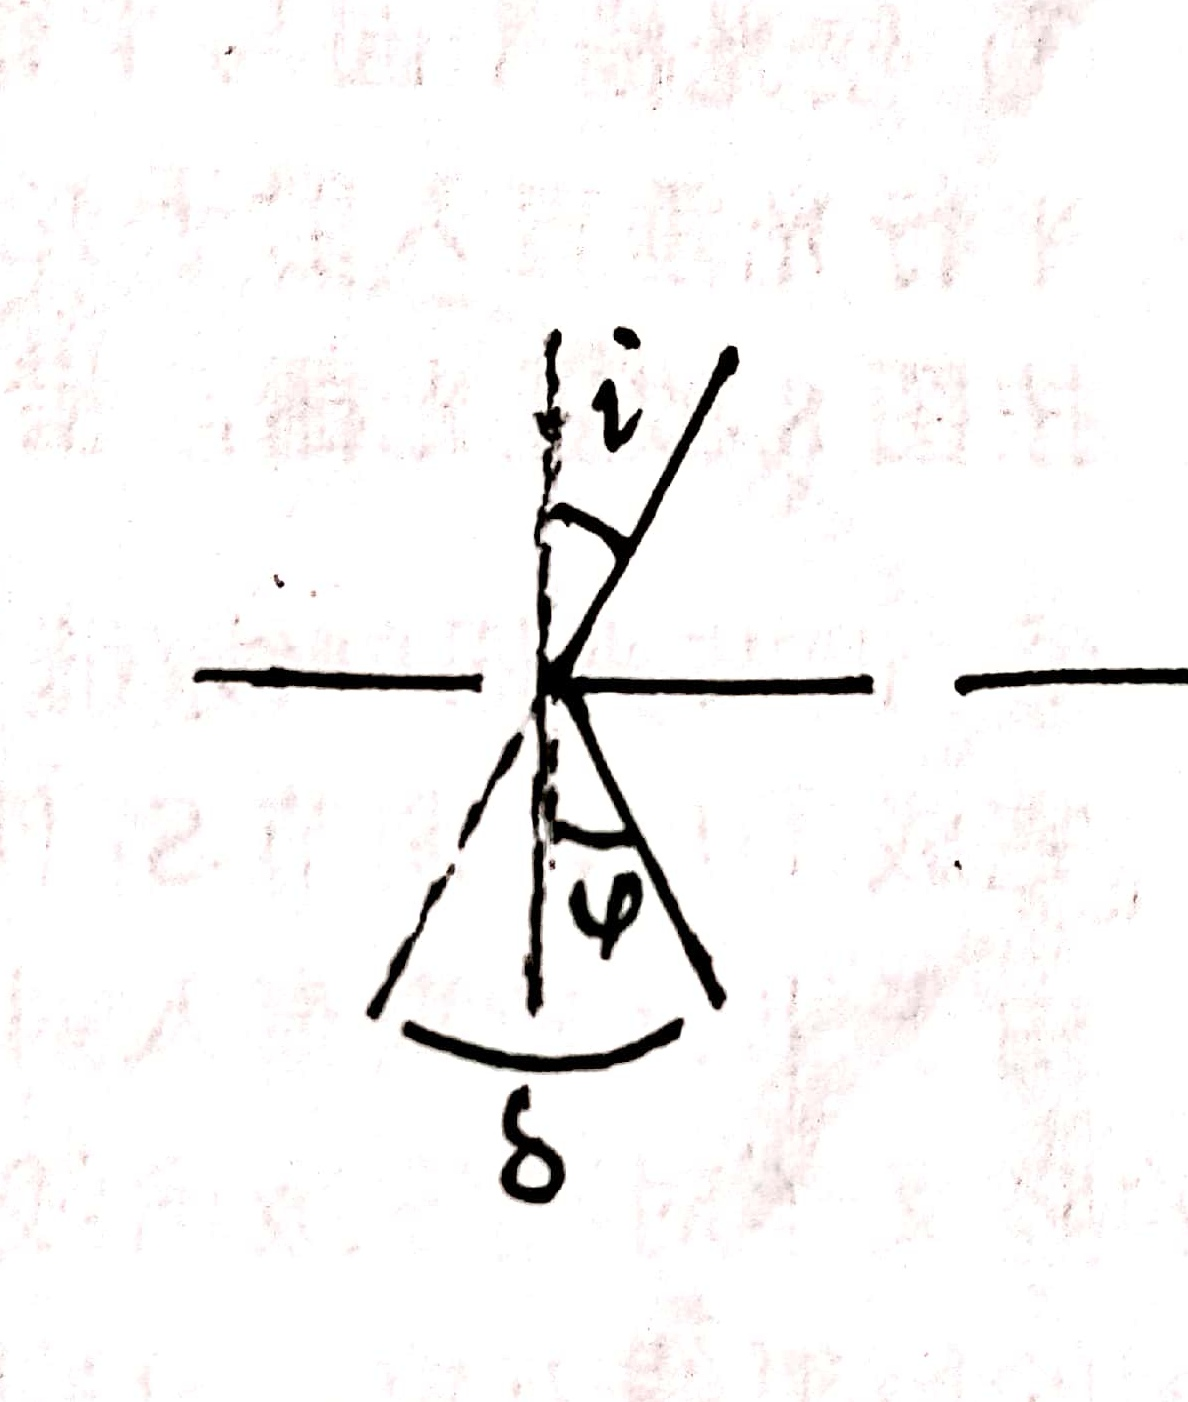
\includegraphics[scale=0.15]{5.jpg}
    \caption{偏向角示意图}
\end{center}\end{figure}
如图,当入射方向和出射方向位于同侧时,有约束条件$d(\sin i+\sin \phi)=m\lambda$,定义$\delta=\phi+i$为偏向角. 由上述两式可以得到
\begin{equation}
    d(\sin(\delta-i)+\sin i)=m\lambda
\end{equation}
我们对上式做全微分,有
\begin{equation}
    d(\cos(\delta-i)d\delta-\cos(\delta-i)di+\cos idi)=0
\end{equation}
因此有
\begin{equation}
    \label{yijiedao}
    \frac{d\delta}{di}=\frac{\cos(\delta-i)-\cos i}{\cos(\delta-i)}
\end{equation}
当偏向角最小时,有$\displaystyle{\frac{d\delta}{di}=0}$,因此有$\cos(\delta-i)-\cos i=0$,这说明$\cos\phi=\cos i$,因此有$\phi=i=\frac{\delta}{2}$. 将此式带入约束条件$d(\sin \phi+\sin i)=m\lambda$,有
\begin{equation}
    2d\sin\frac{\delta}{2}=m\lambda
\end{equation}
因此光波波长可以通过下式获得
\begin{equation}
    \lambda=\frac{2d\sin\frac{\delta}{2}}{m}
\end{equation}
进行实验时,达到最小偏向角条件时,衍射线与初始平行光管光轴方向夹角即为$\delta$. 我们为了提高实验精度,可以测量$2\delta$.\par
具体来说,我们先将载物台上光栅向一个方向旋转,并使望远镜始终追随与旋转方向同侧的第2级外侧黄色衍射线. 当载物台旋转到某处时,衍射线将向旋转方向异侧移动,则该级衍射线能够达到的最外侧方向即最小偏向角条件成立时的衍射光线方向,记录此时望远镜位置$\theta_1$. 与之类似,我们将载物台向另一个方向旋转,并记录最小偏向角条件成立时衍射线方位$\theta_2$,则$2\delta=\Big{|}\theta_2-\theta_1\Big{|}$. 因此有
\begin{equation}
    \lambda=\frac{2d\sin\frac{\delta}{2}}{m}=\frac{2d\sin\frac{|\theta_2-\theta_1|}{4}}{m}
\end{equation}

\subsubsection*{4.2 实验数据及分析}
测量数据如下:m=2
\begin{table}[H]\begin{center}
    \caption{最小偏向角法测量黄光波长数据记录表}
    \begin{tabular}{|c|c|c|c|}
        \hline
        载物台旋转方向&左游标读数$\alpha_1$&右游标读数$\alpha_2$&平均读数$\theta_i=(\theta_1+\theta_2)/2$\\
        \hline
        逆时针旋转&105°07'&285°04'&195°05'\\
        \hline
        顺时针旋转&145°12'&325°10'&235°11'\\
        \hline        
    \end{tabular}
\end{center}\end{table}
则\[\lambda=\frac{2d\sin\frac{|\theta_2-\theta_1|}{4}}{m}=\frac{2\times3329.6\times\sin\frac{|235\degree11'-195\degree05'|}{4}}{2}nm=579.6nm\]
可以看出,测量出的数值与黄光的约定真值$579.1nm$吻合得很好.

\section{思考与讨论}

\paragraph{1.\quad 波长测量的另一种办法}\quad\par
考虑到本实验中各种测量方法均是一次测量,因此,我们不妨设计另一种可以充分利用数据从而测量出波长的办法.\par
由(\ref{yanshe})式知,正入射条件下,波长、衍射角、级数、光栅常数满足$d\sin \phi=m\lambda$,其中$\phi$表示衍射线和法线夹角(以法线到衍射线顺时针旋转为正)则通过测量不同级次$m$对应的$\phi_m$,以$m$为自变量,可以拟合出一条曲线,其斜率为$k=\lambda/d$. 
借用实验内容2.2、2.4中的数据,我们可以进行计算:
\begin{table}[H]\begin{center}
    \caption{直线拟合法测量黄光波长数据记录表}
    \begin{tabular}{|c|c|c|c|c|c|c|}
        \hline
        级数&-3&-2&-1&1&2&3\\
        \hline
        $\phi_m$&-31°27'&-20°20'&9°56'&9°58'&20°20'&31°29'\\
        \hline        
        $\sin\phi_m$&-0.5218&-0.3475&-0.1725&0.1728&0.3475&0.5223\\
        \hline
    \end{tabular}
\end{center}\end{table}
对此组数据利用Excel程序的linest函数对$\sin\phi_m$和$m$做截距为0的最小二乘法直线拟合,设直线斜率为$k$,利用Excel程序的tinv函数计算$p = 0.95$时的$t$因子,可得到:\par
\begin{center}\begin{tabular}{r l}
{斜率}& {$k=0.1739$}\\
{斜率标准偏差}& {$s_k=0.00015$}\\
{t因子}& {$t_{0.95,5}=2.570581836$}\\
{斜率不确定度}& {$U_k=t_{0.95,5}\times s_k = 0.00039$}
\end{tabular}\end{center}
因此,$\sin\phi_m$和$m$拟合得出的直线斜率为$k=(0.1739\pm0.0004)$\par
则
\[\lambda=kd=0.1739\times3329.6nm=579.0nm\]
\[\frac{U_{\lambda}}{\lambda}=\sqrt{(\frac{U_d}{d})^2+(\frac{U_k}{k})^2}=0.2\%\]
\[U_{\lambda}=(\frac{U_{\lambda}}{\lambda})\lambda=1.2nm\]
因此,测得的黄光波长为$(579.0\pm1.2)nm$. 可以看到,该测量的不确定度比2.5中的不确定度$0.2nm$大了一个数量级,我认为主要原因是,分光计是极其灵敏的仪器,仪器误差线小,所以一次测量中不确定度是十分小的;而在多次测量中,可能由于拟合和计算误差过程中多次近似和保留的有效位数有限、低级次时测量不精准、平行光管像存在宽度、实验操作不当改变实验条件、多次测量中出现细小失误等等因素,导致存在较大的误差. 因此该实验设计一次测量而不是多次测量,是有其道理的.\par
除此之外,我还试图用拟合法,不借助绿光约定真值而直接通过斜率和截距算出$d$、$\lambda$等值,但由于$d$与$\lambda$紧密相连,公式$d(\sin i\pm\sin\phi)=m\lambda$中$d$与$\lambda$始终作为外层系数而无法剥离,因此无法直接获得独立的$d$、$\lambda$等值. \par同时,类似的实验一般也都只能通过获得某一约定真值的值从而获得其他量的值. 但若已知某光源的双色或多色光线间存在某种约束条件(如氢原子光谱满足巴耳末系波长计算公式等),便可以用拟合法直接计算相关系数.

\paragraph{2.\quad 关于最小偏向角的进一步讨论和证明}\quad\par
设$\delta$为偏向角,$i$为入射角,由(\ref{yijiedao})式,我们已经得到了
\[\frac{d\delta}{di}=\frac{\cos(\delta-i)-\cos i}{\cos(\delta-i)}=1-\frac{\cos i}{\cos(\delta-i)}\]
当偏向角取极值时,有$\displaystyle{\frac{d\delta}{di}=0}$,由此得到$\cos(\delta-i)=\cos i$,而$\displaystyle{0<\phi=\delta-i<\frac{\pi}{2}}$,$\displaystyle{0<i<\frac{\pi}{2}}$,那么有$\delta=2i$. 然而我们并未证明此处为极大值. 其实要说明这一点也是直接的. 我们只需对上式进行进一步求导,进而得到
\[\frac{d^2\delta}{di^2}=\frac{\sin i\cos(\delta-i)+\cos i\sin(\delta-i)}{\cos^2(\delta-i)}=\frac{\sin\delta}{\cos^2(\delta-i)}\]
考虑到入射角和衍射角位于法线同侧,因此恒有$0<\delta<\pi$,那么$\displaystyle{\frac{d^2\delta}{di^2}}>0$恒成立. 因此$\displaystyle{\frac{d\delta}{di}=0}$,即$\delta=2i$时偏向角为极大偏向角.\par
我们不妨再思考一个问题,在入射角与衍射角分距法线异侧时是否也可以用类似的方法测量光波波长呢?我们先进行如下推导.
\begin{equation}
    d(\sin(\delta-i)-\sin i)=m\lambda
\end{equation}
我们对上式做全微分,有
\begin{equation}
    d(\cos(\delta-i)d\delta-\cos(\delta-i)di-\cos idi)=0
\end{equation}
\begin{equation}
    \frac{d\delta}{di}=\frac{\cos(\delta-i)+\cos i}{\cos(\delta-i)}
\end{equation}
若此时偏向角$\delta$存在极值,则有$\displaystyle{\frac{d\delta}{di}=0}$,那么$\cos(\delta-i)+\cos i=0$. 而另一方面$0<\delta<\pi$,那么$\displaystyle{\frac{d^2\delta}{di^2}}>0$恒成立,即$\cos(\delta-i)+\cos i>0$,这与前面的式子显然是矛盾的,这说明异侧衍射线偏向角不存在极值. 因此,只能测量与入射光同侧衍射线的最小偏向角从而获得光波波长等相关参数.
\paragraph{3.\quad 不确定度的另一种计算方法}\quad\par
我们先进行在2.3原理部分已经推导出
$\displaystyle{d=\frac{m\lambda_{GN}}{\sin\phi_m}}$和$\displaystyle{U_d=\frac{\Delta_{INS}}{2}d \cot\phi_m}$,但实际上
\[{\phi_m=\frac{\phi_2-\phi_1}{2}=\frac{\phi_{21}+\phi_{22}-\phi_{11}-\phi_{12}}{4}}\]
其中$\phi_{21}$、$\phi_{22}$、$\phi_{11}$、$\phi_{12}$才是直接测量量,其不确定度均为$\Delta_{INS}$. 为验证以上不确定度计算的正确性,我们采用这四个量进行不确定度计算. 为此,由$\displaystyle{d=\frac{m\lambda_{GN}}{\sin\frac{\phi_{21}+\phi_{22}-\phi_{11}-\phi_{12}}{4}}}$
\begin{equation}\begin{split}
    U_d&=
    \sqrt{(\frac{\partial d}{\partial \phi_{11}}U_{\phi_{11}})^2+(\frac{\partial d}{\partial \phi_{12}}U_{\phi_{12}})^2+(\frac{\partial d}{\partial \phi_{21}}U_{\phi_{21}})^2+(\frac{\partial d}{\partial \phi_{22}}U_{\phi_{22}})^2}\\
    &=\sqrt{
        (\frac{m\lambda_{GN}\cos\phi_m}
        {\sin^2\phi_m}\frac{U_{\phi_{11}}}{4})^2+
        (\frac{m\lambda_{GN}\cos\phi_m}
        {\sin^2\phi_m}\frac{U_{\phi_{12}}}{4})^2+
        (\frac{m\lambda_{GN}\cos\phi_m}
        {\sin^2\phi_m}\frac{U_{\phi_{21}}}{4})^2+
        (\frac{m\lambda_{GN}\cos\phi_m}
        {\sin^2\phi_m}\frac{U_{\phi_{22}}}{4})^2
    }\\
    &=\sqrt{4\frac{m\lambda_{GN}\cos\phi_m\Delta_{INS}}{16\sin^2\phi_m}}\\
    &=\frac{\Delta_{INS}}{2}d \cot\phi_m
\end{split}\end{equation}
这与我们之前通过间接计算$\phi_1$、$\phi_2$不确定度获得的最终不确定度一致,验证了该方法的正确性. 事实上,类似通过直接测量量获得中间量不确定度的方法,只要直接测量量关于中间量都是一次的,那么均是正确的,证明均与上类似. 所以,在$U_{\lambda}$的计算中我们也采用了类似的办法,不再赘述.
\paragraph{4.\quad 为什么实验中测量$2\phi_m$}\quad\par
由思考与讨论3中不确定度的推导我们可以看出,若测量m级衍射角方位$\phi_1=(\phi_{11}+\phi{12})/2$和0级主极大方位$\phi_0=(\phi_{01}+\phi_{02})/2$,那么就有$\displaystyle{d=\frac{m\lambda_{GN}}{\sin(\phi_1-\phi_0)}=\frac{m\lambda_{GN}}{\sin\frac{\phi_{11}+\phi_{12}-\phi_{01}-\phi_{02}}{2}}}$,为此
\begin{equation}\nonumber\begin{split}
    U_d&=
    \sqrt{(\frac{\partial d}{\partial \phi_{01}}U_{\phi_{01}})^2+(\frac{\partial d}{\partial \phi_{02}}U_{\phi_{02}})^2+(\frac{\partial d}{\partial \phi_{11}}U_{\phi_{11}})^2+(\frac{\partial d}{\partial \phi_{12}}U_{\phi_{12}})^2}\\
    &=\sqrt{
        (\frac{m\lambda_{GN}\cos\phi_m}
        {\sin^2\phi_m}\frac{U_{\phi_{01}}}{2})^2+
        (\frac{m\lambda_{GN}\cos\phi_m}
        {\sin^2\phi_m}\frac{U_{\phi_{02}}}{2})^2+
        (\frac{m\lambda_{GN}\cos\phi_m}
        {\sin^2\phi_m}\frac{U_{\phi_{11}}}{2})^2+
        (\frac{m\lambda_{GN}\cos\phi_m}
        {\sin^2\phi_m}\frac{U_{\phi_{12}}}{2})^2
    }\\
    &=\sqrt{4\frac{m\lambda_{GN}\cos\phi_m\Delta_{INS}}{4\sin^2\phi_m}}\\
    &=\Delta_{INS}d \cot\phi_m
\end{split}\end{equation}
其不确定度明显比通过$2\phi_m$来计算要大,因此一般采用$2\phi_m$测量而不直接通过m级和0级衍射线测量. 除此之外,还有一个重要的原因是:进行实验时,平行光管的像位置有可能会受到轻微扰动,从而直接对入射角和衍射角均产生干扰. 而通过$2\phi_m$测量法,平行光管位置受到扰动,则干扰的仅仅是入射角,而入射角又是小角,变化为可忽略的小量,因此测量结果受到的影响也略低一些.

\paragraph{5.\quad 正入射、斜入射或最小偏向角法中$\displaystyle{\Big{|}\frac{\sin\theta_1-\sin\theta_2}{2}\Big{|}}$与$\displaystyle{\sin\frac{|\theta_1|+|\theta_2|}{2}}$是否等效}\quad\par
$\theta_1$、$\theta_2$分别定义为$\pm m$级衍射条纹与0级主极大间的方位夹角. 考虑到正入射、最小偏向角法两种方法中,$\pm m$级衍射条纹测量时均为对称的,即有$|\theta_1|=|\theta_2|$,设$\theta_1<0<\theta_2$,那么$\displaystyle{\Big{|}\frac{\sin\theta_1-\sin\theta_2}{2}\Big{|}=sin\theta_2=\sin\frac{|\theta_1|+|\theta_2|}{2}}$,即二者等效. 而对于斜入射,由于衍射角并不关于法线对称,因此没有$|\theta_1|=|\theta_2|$等式关系,也就没有二者等效这一结论.
\paragraph{6.\quad 可能导致误差的因素}\quad\par
\textbf{i.)}绿光的约定真值与实际值有一定偏差,以此算出的$d$、$\lambda$等诸多物理量均会出现误差.\par
\textbf{ii.)}由于平行光管狭缝存在一定宽度,所以它的像以及各级衍射线不是一条严格的线而是一个斑. 衍射斑存在宽度,则测量时不能严格测得主极大发生的方位,因此存在一定误差.\par
\textbf{iii.)}由于光栅制作工艺限制,刻线未必水平且未必等距\par
\textbf{iv.)}进行实验时,诸多实验条件可能无法十分严格,如望远镜或平行光管未水平、小平台未水平、未垂直等,均可能对实验造成较大的误差.
入射\par
\textbf{v.)}实验操作时,可能会受到一定扰动,如载物台最上层无法固定,轻微碰触乃至于周围同学拍动桌子都可能对其造成一定的干扰,因此也可能产生误差.\par
\textbf{vi.)}各种光学实验依靠人眼观察现象,但视差不能完全消除. 且对于近视的同学来说,卸掉眼镜和不卸眼镜都可能对看到的实验现象产生巨大的影响,这也是影响因素之一.\par
\textbf{vii.)}最小偏向角法测量过程中,由于最小偏向角的方位难以寻找,很难恰好将望远镜十字叉丝竖线对准最小偏向角发生时衍射条纹的位置,因此可能会出现误差.\par
\textbf{viii)}刻度盘除偏心差外还有一些由于盘形状不规则而产生的误差\par
以上均为系统误差,实验过程中,许多数据均为单次测量,也难免会因为人为因素而产生随机误差. 因此,综合考虑以上因素,本次实验的测量数据与理论值吻合得较好.

\vspace{2em}
\section{实验结论}

在本次实验中,我们首先进行分光计工作条件的调节:调节望远镜光轴垂直分光计主轴,并保证望远镜能够看到平行光管无视差的像,然后需要调节光栅平面与平行光管光轴垂直,这就完成了工作条件的调节. 其次,我们采用正入射法,并利用绿光的约定真值测得光栅常数,然后在此基础上利用正入射法、斜入射法和最小偏向角法测量光波波长,在用前两种方法测量时,还需用自准直法保证一定的实验条件. 最后,我们测得光栅常数为$d=(3329.6\pm0.9)nm$,用三种方法测得的黄光波长分别为$579.4nm$、$580.2nm$和$579.6nm$. 这些测量值与黄光的约定真值$579.1nm$吻合得较好,进一步验证了实验方法和操作的正确性.\par
在进行本次试验过程中,我掌握了分光计的使用和调节方法,进一步巩固了进行物理实验的步骤和基本方法. 在后续处理数据、撰写实验报告的过程中,我还进一步对光栅衍射中正入射、斜入射和最小偏向角等相关理论知识有了进一步理解,同时回顾了实验误差的分析、不确定度的计算等相关知识.
\newpage
\section{原始数据}
\begin{figure}[H]\begin{center}
    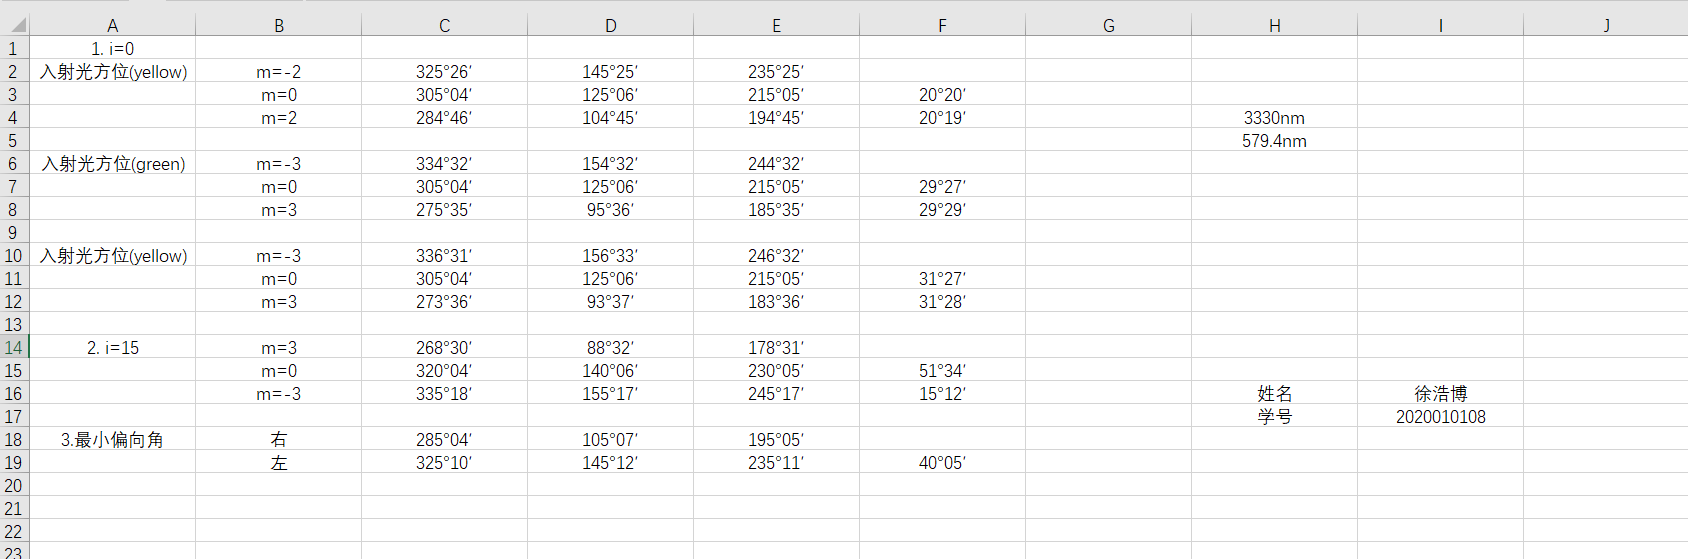
\includegraphics[scale=0.5]{data.PNG}
\end{center}\end{figure}
\end{document}